%%% Template originaly created by Karol Kozioł (mail@karol-koziol.net) and modified for ShareLaTeX use

\documentclass[a4paper,11pt]{article}

\usepackage[T1]{fontenc}
\usepackage[spanish]{babel}
\usepackage[utf8]{inputenc}
\usepackage{graphicx}
\usepackage{xcolor}
\usepackage{wrapfig}

\renewcommand\familydefault{\sfdefault}
\usepackage{tgheros}
\usepackage[defaultmono]{droidmono}

\usepackage{amsmath,amssymb,amsthm,textcomp}
\usepackage{enumerate}
\usepackage{multicol}
\usepackage{tikz}

\usepackage{geometry}
\geometry{total={210mm,297mm},
left=25mm,right=25mm,%
bindingoffset=0mm, top=20mm,bottom=20mm}


\linespread{1.3}

\newcommand{\linia}{\rule{\linewidth}{0.5pt}}

% custom theorems if needed
\newtheoremstyle{mytheor}
    {1ex}{1ex}{\normalfont}{0pt}{\scshape}{.}{1ex}
    {{\thmname{#1 }}{\thmnumber{#2}}{\thmnote{ (#3)}}}

\theoremstyle{mytheor}
\newtheorem{defi}{Definition}

% my own titles
\makeatletter
\renewcommand{\maketitle}{
\begin{center}
\vspace{2ex}
{\huge \textsc{\@title}}
\vspace{1ex}
\\
\linia\\
\@author \hfill \@date
\vspace{4ex}
\end{center}
}
\makeatother
%%%

% custom footers and headers
\usepackage{fancyhdr}
\pagestyle{fancy}
\lhead{}
\chead{}
\rhead{}
\lfoot{Entrega \textnumero{}  4 - Proyecto Seguridad Informática}
\cfoot{}
\rfoot{Página \thepage}
\renewcommand{\headrulewidth}{0pt}
\renewcommand{\footrulewidth}{0pt}
%

% code listing settings
\usepackage{listings}
\lstset{
    language=Python,
    basicstyle=\footnotesize,
    frame=.2,
  xleftmargin=.2\textwidth, xrightmargin=.2\textwidth,
    basicstyle=\ttfamily\small,
    columns=fixed,
    extendedchars=true,
    breaklines=true,
    tabsize=6,
    prebreak=\raisebox{1ex}[1ex][1ex]{\ensuremath{\hookleftarrow}},
    showspaces=false,
    showstringspaces=false,
    keywordstyle=\color[rgb]{0.627,0.126,0.941},
    commentstyle=\color[rgb]{0.133,0.545,0.133},
    stringstyle=\color[rgb]{01,0,0},
    captionpos=t,
    escapeinside={\%*}{*)}
}

%%%----------%%%----------%%%----------%%%----------%%%

\begin{document}

\begin{titlepage} % Suppresses displaying the page number on the title page and the subsequent page counts as page 1
	
	\raggedleft % Right align the title page
	
	\rule{1pt}{\textheight} % Vertical line
	\hspace{0.05\textwidth} % Whitespace between the vertical line and title page text
	\parbox[b]{0.75\textwidth}{ % Paragraph box for holding the title page text, adjust the width to move the title page left or right on the page
	 \begin{tabularx}{\linewidth}{}
    \makecell{
\includegraphics[height=2cm]{logo}}
     \end{tabularx}
     \bigskip
     \vfill
		{\Huge\bfseries Entrega \textnumero{} 4 Proyecto\\[0.5\baselineskip] Seguridad ~ Informática}\\[2\baselineskip] % Title
		{\large\textsc{Auditoria de la Aplicación y}}\\
		{\large\textsc{Decompilación }}\\[1\baselineskip] % Subtitle or further description
		{\normalsize\textit{Camilo Zepeda Hoffmann}} % Author name, lower case for consistent small caps
		
		\vspace{0.5\textheight} % Whitespace between the title block and the publisher
		
		{\noindent Profesor~ Maximiliano~Vega\plogo}\\[\baselineskip] % Publisher and logo
		{\normalsize\textit{02 de Noviembre 2017}}
	}

\end{titlepage}


\section{Resumen}

Ya en conocimiento de los datos y archivos encontrados se realizan pruebas asociadas a la captación de paquetes, utilizando prácticas de man-in-the-middle y herramientas pertienentes que efecten la recopilación de los nombrados paquetes.




\section{Pruebas y Herramientas}
Se realizan pruebas del tipo interceptoras, con tal de captar información sensible utilizando falseos de certificados y Wireshark. 
Entonces para determinar lograr un mayor comprendimiento de los pasos realizados, se nombra:



\begin{itemize}
    \item \textbf{Paso 1}: es necesario generar una variable ambiente del tipo \textbf{PATH} que contenga de nombre SSL y la ruta del archivo a efectuar: 
    
    \begin{verbatim}
       C\\ruta\\ruta\\ sslkeylog.log
    \end{verbatim}

    donde \textbf{sslkeylog.log} corresponde al archivo contenedor de los certificados ssl falsificados. Lo anterior se describe en la siguiente imagen:
    
    \begin{figure}[!h]
    \centering
    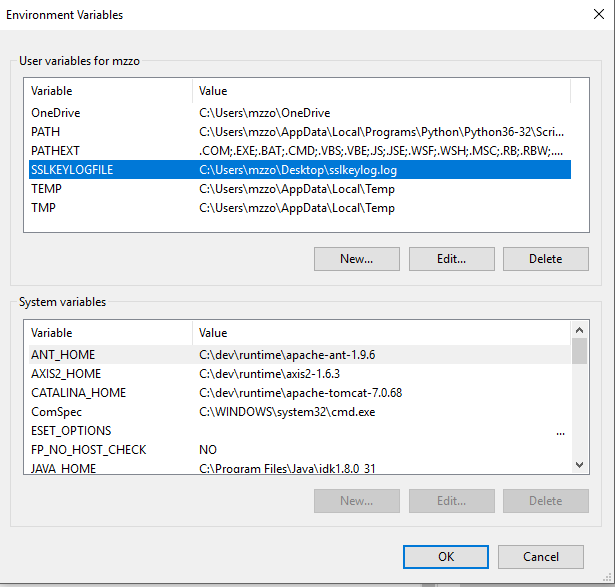
\includegraphics[scale=0.5]{sslpath.png}
    \label{fig:my_label}
    \end{figure}
    
    Al generar la variable de ambiente dentro del entorno del sistema operativo, se genera de manera automáticamente el archivo nombrado, el cual contiene:
    \newpage
    \begin{figure}[!h]
    \centering
    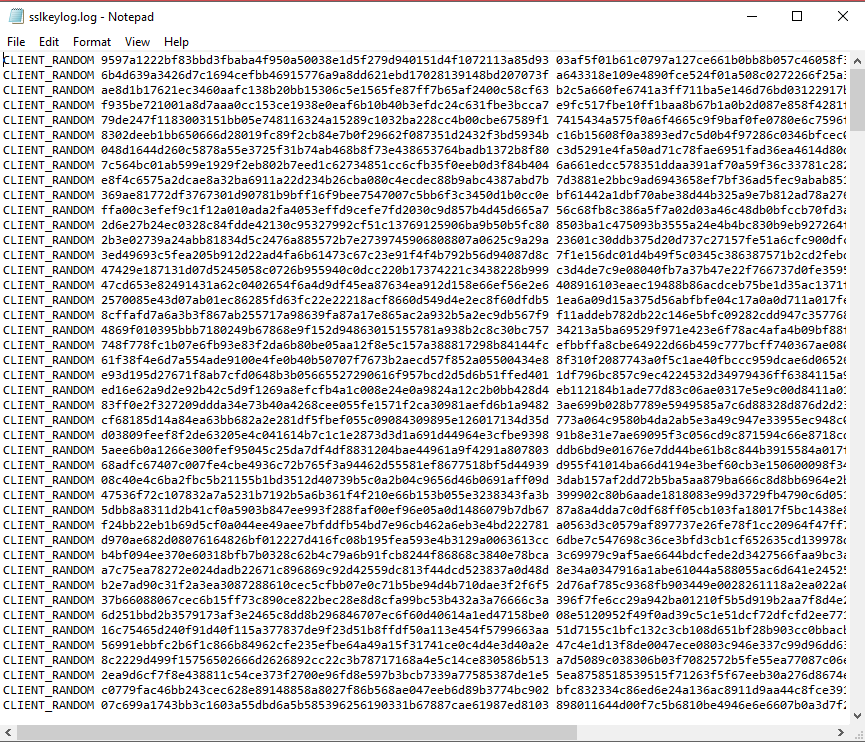
\includegraphics[scale=0.4]{ssllog.png}
    \label{fig:my_label}
    \end{figure}
        
    
    \item \textbf{Paso 2}: ya extraído el archivo anteriormente mencionado, se procede a adjuntar los certificados a herramienta \textbf{WireShark}, con tal de generar una captación y evaluación real del desempeño de los certificados. A continuación se presenta lo descrito:
    
     \begin{figure}[!h]
    \centering
    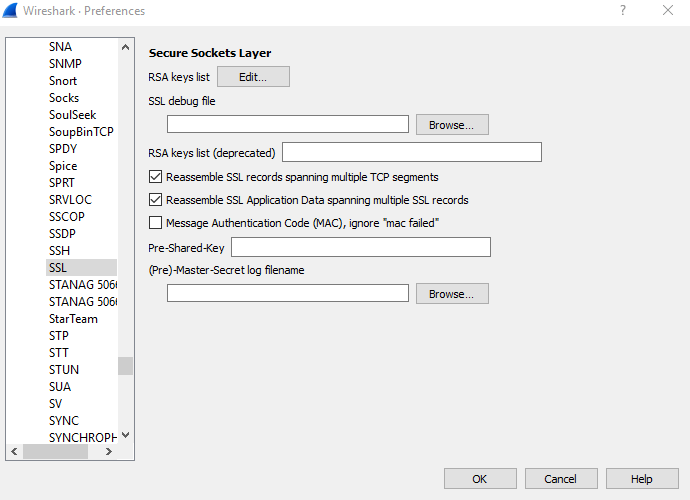
\includegraphics[scale=0.5]{wiressl.png}
    \label{fig:my_label}
    \end{figure}
    
 
Es necesario proveer la ruta especifica en donde se encuentra el archivo generado por el PATH, de tal manera que trabajen como decifradores de las request generadas al hacer man-in-the-middle, trabajando entonces sobre los paquetes captados al probar la aplicación.
    
    \item \textbf{Paso 3}: Una vez realizado los pasos anteriores se procede generar la prueba de captación de paquetes, para lo cual fue necesario implementar el computador como emisor de conexión WIfi recepcionado por el dispositivo móvil contenedor de la aplicación. Entonces se obtiene:
    
    \newpage
  
    
    \begin{figure}[!h]
    \centering
    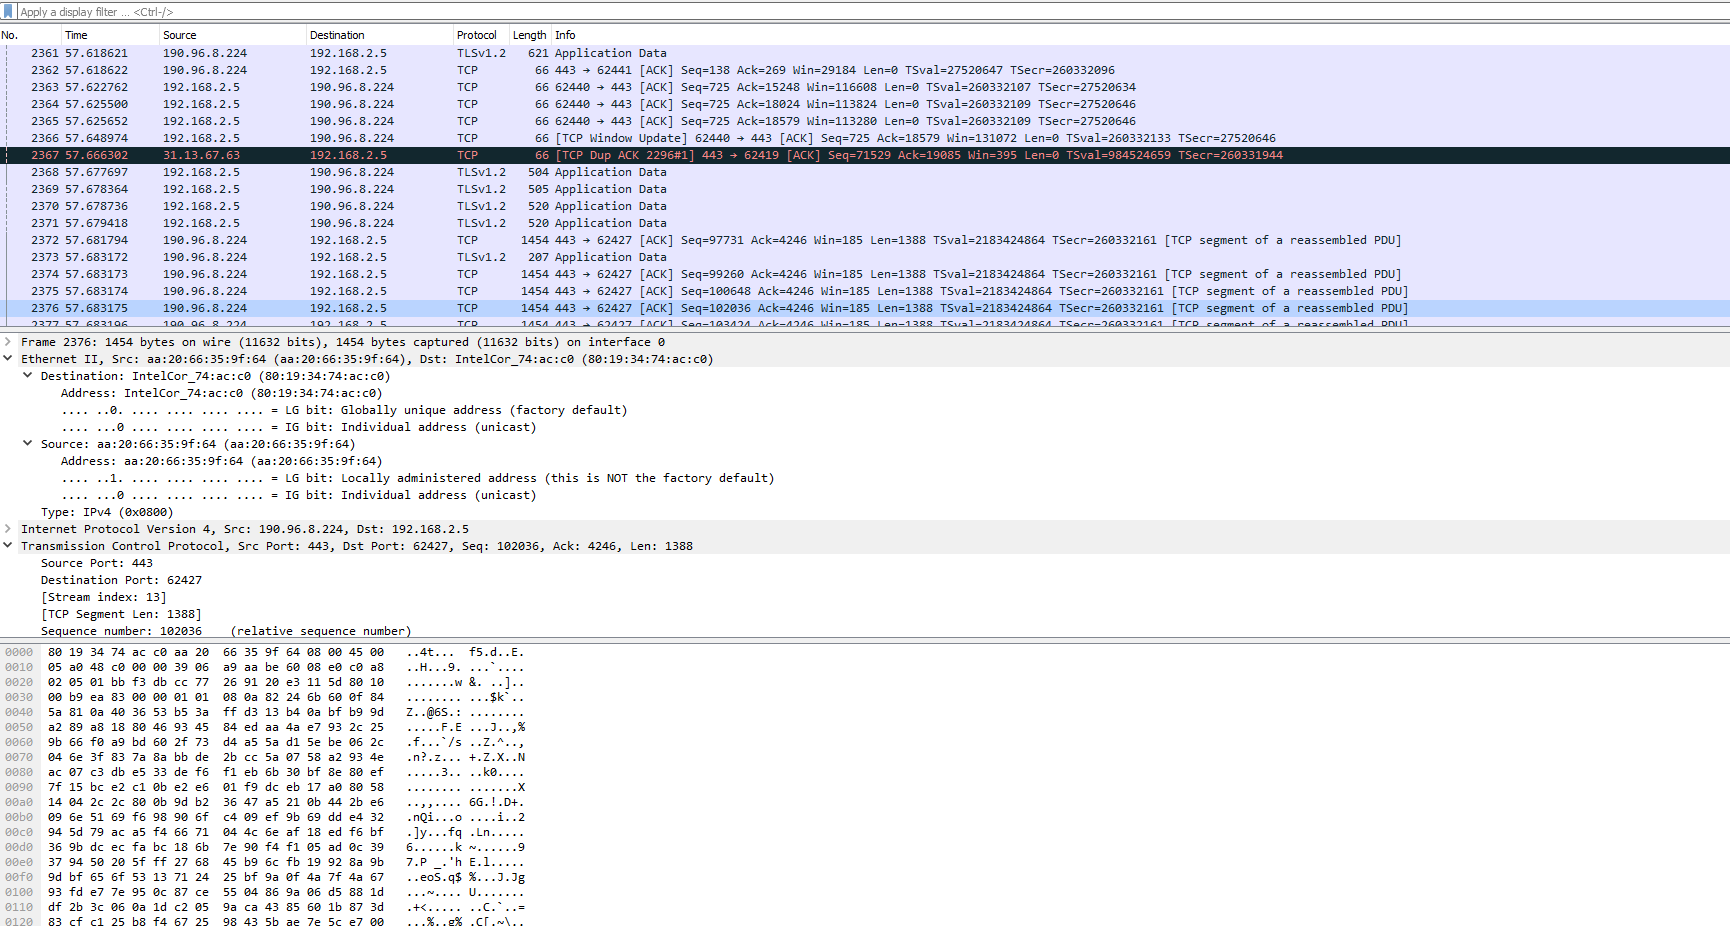
\includegraphics[scale=0.27]{paqueteswiressl.png}
    \label{fig:my_label}
    \end{figure}
    
    La figura anterior describe la prueba asociada, dando a conocer los paquetes e intentando descifrar los archivos y request solicitadas, por medio de los certificados generados. Otro ejemplo concluyente de los resultados fue:
    
    \begin{figure}[!h]
    \centering
    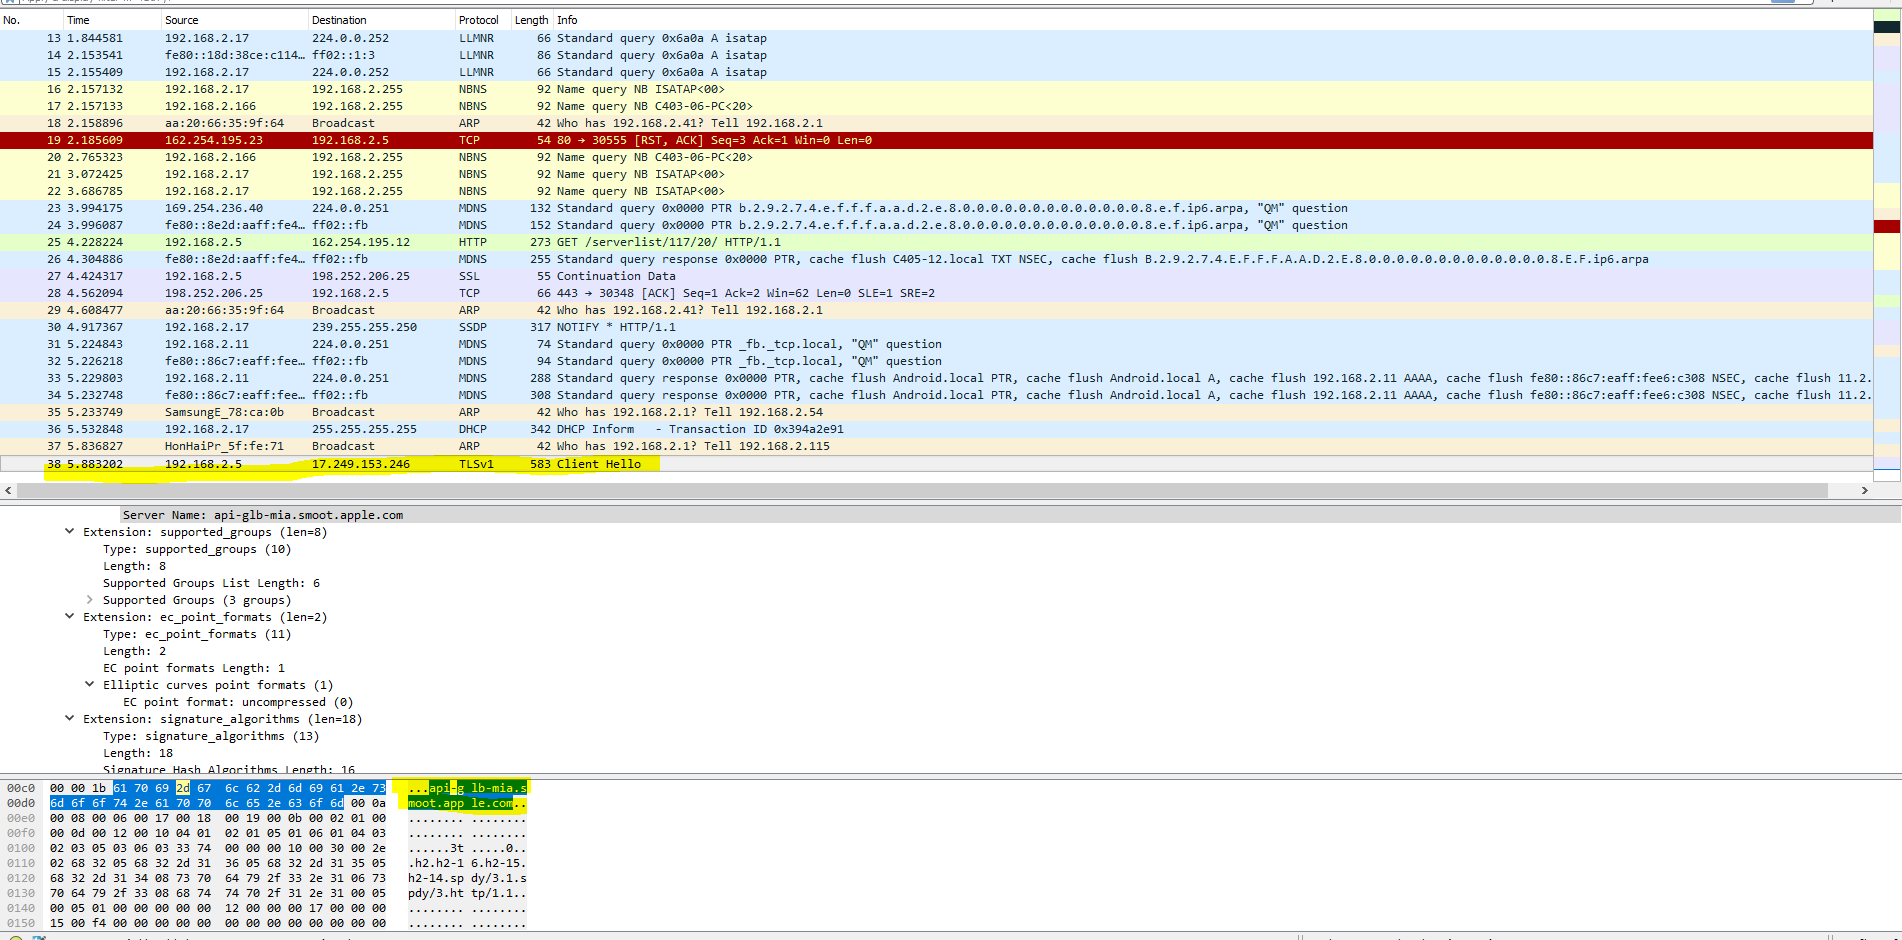
\includegraphics[scale=0.25]{paquetelectura.png}
    \label{fig:my_label}
    \end{figure}
    
    Es posible apreciar lectura de los paquetes, entregando paquetes del tipo TCP y CLIENT HELLO, de la cuál se adjunta una recepción del paquete mayormente ilegible, pero aún así, no se encuentra información consistente y tangible de las respuestas. Lo que implica que no es posible captar la información de los usuarios o bien sentencias explotables, dando a entender que los certificados generados no proveen de información y por tanto de utilidad.
 
    
    
\end{itemize}


\subsection{Propuestas para Quintp Incremento}

Con el fin de lograr una mayor comprensión de lo propuesto se define el siguiente listado.

\begin{itemize}
    \item Analizar en profundidad las funciones Internas React, depurando la información.
    \item Generar certificados SSL para el desarrollo de Man-in-the-Middle 
    \item Buscar posibles Scripts utilizados para robar información.
    \item Utilizar herramientas de OpenSSL con tal de generar nuevos certificados ssl, capaces de captar información de utilidad.
\end{itemize}



\newpage










\begin{thebibliography}{1}
\bibitem{Oauth}
A. Plaza, "Un fallo de seguridad en Instagram muestra la vulnerabilidad de las cuentas | Hipertextual", Hipertextual, 2017. [Online]. Available: \url{https://hipertextual.com/2013/05/fallo-de-seguridad-en-instagram}. [Accessed: 11- Oct- 2017].


\bibitem{cuentas}
"La posibilidad de usar varias cuentas en Instagram presenta un fallo de seguridad - TreceBits", TreceBits, 2017. [Online]. Available: \url{http://www.trecebits.com/2016/02/16/la-posibilidad-de-usar-varias-cuentas-en-instagram-presenta-un-fallo-de-seguridad/}. [Accessed: 11- Oct- 2017].

\bibitem{hack}
"El hackeo a Instagram, más grave de lo esperado: 6 millones de cuentas", ADSLZone, 2017. [Online]. Available: \url{https://www.adslzone.net/2017/09/02/el-hackeo-instagram-mas-grave-de-lo-esperado-6-millones-de-cuentas/}. [Accessed: 11- Oct- 2017].

\bibitem{appirater}
https://www.buzztouch.com/forum/thread.php?tid=B60C6EE41CD7D289048B0F4

\bibitem{appirater2}
https://github.com/arashpayan/appirater

\bibitem{reachability}
https://iphoneros.com/44273/asi-es-el-modo-reachability-para-poder-utilizar-el-iphone-6-plus-con-una-sola-mano-video

\bibitem{curl}
https://curl.haxx.se/docs/history.html

\end{thebibliography}

\newpage



\end{document}
